\documentclass[11pt, letterpaper]{article}
\usepackage[utf8]{inputenc}
\usepackage[letterpaper, margin=0.5in]{geometry}
\usepackage{amsmath}
\usepackage{amssymb}
\usepackage{amsthm}
\usepackage{graphicx}
\usepackage{listings}
\usepackage[font=scriptsize]{caption}
\usepackage{subcaption}
\usepackage{xcolor}

\newtheorem{lemma}{Lemma}
\newcommand{\indep}{\perp \!\!\! \perp}

\definecolor{codegreen}{rgb}{0,0.6,0}
\definecolor{codegray}{rgb}{0.5,0.5,0.5}
\definecolor{codepurple}{rgb}{0.58,0,0.82}
\definecolor{backcolour}{rgb}{0.95,0.95,0.92}

\lstdefinestyle{mystyle}{
    backgroundcolor=\color{backcolour},   
    commentstyle=\color{codegreen},
    keywordstyle=\color{magenta},
    numberstyle=\tiny\color{codegray},
    stringstyle=\color{codepurple},
    basicstyle=\ttfamily\footnotesize,
    breakatwhitespace=false,
    texcl=true,
    mathescape=true,
    breaklines=true,                 
    captionpos=b,                    
    keepspaces=true,                 
    numbers=left,                    
    numbersep=5pt,                  
    showspaces=false,                
    showstringspaces=false,
    showtabs=false,                  
    tabsize=2
}

\lstset{style=mystyle}
\graphicspath{ {../statics/} }
\captionsetup{justification=raggedright, singlelinecheck=false}

\author{Ryan Tang}
\title{STA 532 HW 6}
\date{March 5th 2023}

\begin{document}
\maketitle

\section{Ex 3-1}
\paragraph{(a)}
Generally, assuming the $H_o$ is true, the p-value follows a uniform distribution. It is shown below. Let $F(.)$ be the cdf function of distribution and $T(X) = t$ be the test statistics. Our binomial cases simplify the test statistics to $T(X) = x_{obs}$.
\begin{align*}
    p &= P(T(X) \ge t | H_o) \\
        &= 1 - P(T(X) < t | H_o) \\
        &= 1 - F_{H_o}(t) \\
    F_{H_o}(t) &= 1 - p \\
    p_{H_o}(p) &= \frac{\partial}{\partial t} F_{H_o}(t) = 1 \thicksim U(0, 1)
\end{align*}

\paragraph{(b)}
It has become obvious due to the proof of (a) that the test rule $\delta(x) = $ "reject $H_o$ if $p < \alpha$, $\alpha \in (0, 1)$". Because assuming the $H_o$ is true, the chance we get it wrong by following the rule $delta(x)$ is $\alpha$ asymptotically, which is the Type I error.

\paragraph{(c)}
Now, we have the data $n=500, x = 300$ under our binomial opinion poll case. Assuming we reject the $H_o$ at $\alpha = 0.00001$, the corresponding $\beta$ ratio can be found by first finding the critical value $c$.
\begin{align*}
    X &\thicksim Binom(n=500, p=\phi) \\
    \alpha &= 0.00001 = P(X \ge x_{obs} | \phi = 0.5) \\
    c &= F^{-1}(q=0.00001, n=500, \phi=0.5) = 298 \\
    \beta &= P(X \le c | \phi = 0.6) \approx 0.44
\end{align*}

\paragraph{(d)}
Here we fix the test rule from (c), $\delta(x) = $ "reject $H_o$ if $p < \alpha, \alpha=0.00001, \beta=0.44$". Then, we can compare it with a different test rule under the same binomial assumption, $\delta'(x) = $ "reject $H_o$ if $p < \alpha, \alpha=0.05, \beta=0.002$". Rejecting or accepting either rule gives an entirely different interpretation. Especially the former is much more conservative than the latter. Hence, due to conservatism, the change of Type II error is inflated at the pre-determined $H_o$ and $H_1$. 


\section{Ex 3-3}
\paragraph{(d)}
The conditional p-value $p = P(T(X) \ge t|H_o)$ should follow a uniform distribution because the $H_o$ and the corresponding test statistics are sufficient, which follows the same argument in the proof from 3.1(a). The maximum operator in Fisher's p-value drops because of the conditional. However, the complication comes in due to the composition and unconditional p-value "$\mathop{\max}_{P\in \mathcal{P}_o} P(T(X) \ge t)$", which can be multi-modal weirdly shaped.

\newpage
\section{Ex 3-4}
We like to experiment to see if there is a trend on the tropical cyclone annual count dataset, $X =(X_1, X_2, \dots, X_n)$. Under Fisher's framework, we have the null hypothesis $H_o: X_i \thicksim_{iid} \text{Poisson}(\alpha)$. And the test statistics, $T=\frac{W}{\bar{X}+1/n}, W=\frac{1}{n(n+1)}\sum_j^n jX_j$. The sufficient statistics for the experiment are also collected, $n=100, W = 4.69, \bar{X}=8.77, T=0.534$. Hence, Fisher's p-value equals $\max_{\alpha>0} P(T\ge 0.534|\alpha)$.

\paragraph{(a)}
First, since it maximizes over all possible $\alpha$, we run a Monte Carlo to estimate the p-value, and the distribution of p-values against various $\alpha$ is plotted below. We can see that Fisher's p-value is maximized when $\alpha \approx 0.162, p = 0.172$. This is the p-value that would be reported under the framework.

\begin{figure*}[!h]
  \centering
  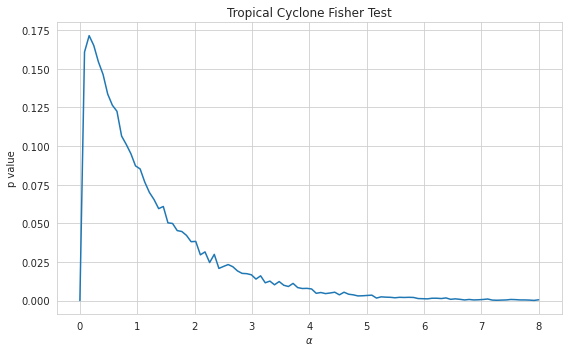
\includegraphics[width=0.6\textwidth]{hw6-1.png}
  \captionsetup{justification=centering}
\end{figure*}

\paragraph{(b)}
Continuing from (a), Fisher's p-value is super conservative, which tries to minimize the worst-case scenario. Over the all possible range of $\alpha \in [0, \infty)$ we would report $p = 0.172$. However, if we restrict $\alpha \in [5, 30]$, and rerun the above simulation, the corresponding p-value becomes $p = 0.0037$, which centers around the smallest possible $\alpha$.

\paragraph{(c)}
Alternatively, we can calculate the plug-in p-value $P(T>0.534|\alpha=8.77) = 0.00018$, where $\alpha=8.77$ is estimated from the sample average. I think it makes sense and is more reasonable than (a). However, there are two cons. This method doesn't consider the uncertainty of the sample mean estimate. Second, the data might be generated from an entirely different, unknown, complicated underlying process but look similar to an IID Poisson, ie. autocorrelation, seasonally, nonlinear transitions. In other words, the plug-in p-value only considers the limited space under the null hypothesis $\mathcal{P}_o \in \mathbb{P}$.

\paragraph{(d)}
Of course, alternatively, we can report the conditional p-value $p = P(T>0.534|R=X_1+ \dots +X_n)$. As we know, the vector $X \thicksim \text{Multinomial}(R, \frac{1}{n}\mathbf{1}_n), R=\bar{X}\cdot n=877, n = 100$. In other words, the sufficient statistics $R$ is the sum of all $X_j$. Lastly, the conditional p-value can be estimated using Monte Carlo $P(T>0.534|R) = 0.0001$. Compared to the plug-in p-value, the conditional p-value is more comprehensive; it is a weighted average of all possible $\alpha$ under the $H_o$ because we marginalized $\alpha$ out by conditioning on the sufficient statistics. Either way, (c) or (d), both signals reject the null hypothesis and suggest a trend in the dataset.

\newpage
\section{Ex 3-5}
\paragraph{(a)}
Here we first define the confidence interval rule $\gamma^B(X) = [\underline{\gamma}^B(X), \overline{\gamma}^B(X)]$ for the 2.5th and 97.5th percetile of $p(\phi|X)$ posterior or the prior $p(\phi)$. We know Beta is the conjugate prior to the Binomial distribution. With the prior $\phi \thicksim Beta(1, 1)$, the posterior $\phi|X \thicksim Beta(x + 1, n-x+1)$.

Now, we are interested in the prior-averaged coverage $\gamma^B$. We prove it is indeed a 95\% confidence rule. Quick note, $\gamma^B$ follows $Beta(1,1)$'s 95th confidence interval, which is a uniform distribution.
\begin{align*}
    \phi &\thicksim U(0, 1) \\
    p(\phi) &= 1 \\
    \int \text{coverage}(\gamma^B|\phi) p(\phi) d\phi
        &= E[E[\text{coverage}(\gamma^B, \phi)|\phi]] \\
        &= E[Pr(\underline{\gamma^B} \le \phi \le \overline{\gamma^B})|\phi] \\
        &= E[0.95|\phi] \\
        &= 0.95
\end{align*}

\paragraph{(b)}
Going further with the Bayesian confidence interval on the posterior $\phi|X \thicksim Beta(x+1, n-x+1)$. Here, we plot the Monte Carlo estimate of the coverage ratio for each $\phi^*$. Under $n=500$ sample size, the posterior confidence interval coverage does as well as we expected, except on two special points, $\phi^* = 0, 1$. Due to the bias in the prior, we need $n \rightarrow \infty$ to have the 95th posterior confidence interval include 0 or 1. Other than these two singularities, I would say the confidence coefficient of $\gamma^B = 0.95$.
\begin{figure*}[!h]
  \centering
  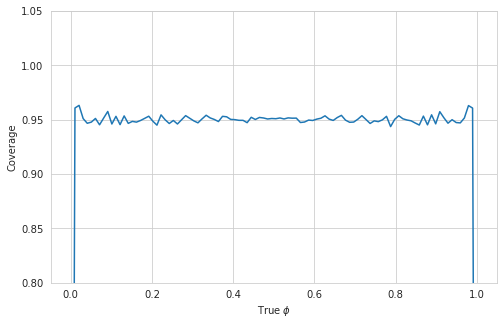
\includegraphics[width=0.6\textwidth]{hw6-2.png}
  \captionsetup{justification=centering}
\end{figure*}

\paragraph{(c)}
Certainly, the prior of $\phi$ plays a significant role in determining the usefulness of the confidence interval rule $\gamma^B$. Two salient, extreme, examples are, taking $n=500$, priors either with $\phi \thicksim Beta(\infty, 1)$ or $\phi \thicksim Beta(1, \infty)$. It is simple to see the coverage ratio of these two priors will be a singularity of 100\% when the true $\phi^*$ is either 0 or 1 and 0\% coverage everywhere else.

\end{document}